\section{Moat band spin liquids and emergent gauge field and anyon}
%----------------------------------------------------------------------------------------
\subsection{Moat band systems}
%----------------------------------------------------------------------------------------
\begin{frame}{Moat band}
\begin{columns}
    
    \begin{column}{0.4\textwidth}
        \centering
        \begin{block}{}%{Moat band}
        \begin{itemize}
            \item Moat band has degenerate energy minima along a closed line in the Brillouin zone
            \item Unlike the flat band systems, higher energy states also play a role in the system even for low energy physics
        \end{itemize}
        \end{block}
    \end{column}
    
    \begin{column}{0.5\textwidth}  % Adjusted the column width
        \centering
        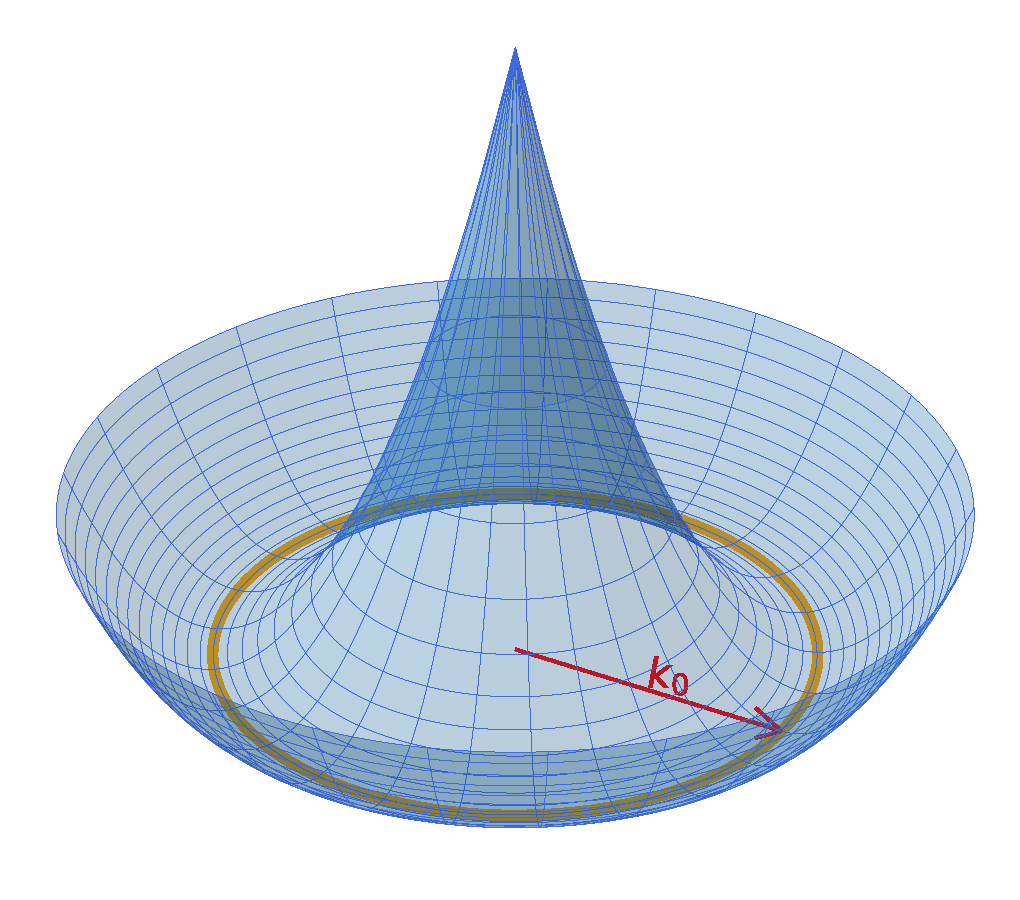
\includegraphics[width=0.7\textwidth]{figs/CSL/moatband.pdf}
        
        $E(\mathbf{k}) = (|\mathbf{k}| - k_0)^2$
    \end{column}
\end{columns}
\end{frame}

%----------------------------------------------------------------------------------------

\subsection{Frustrated $J_1$ - $J_2$ model}

\begin{frame}{$J_1$ - $J_2$ $XY$ model on honeycomb lattice}
\begin{columns}
    \begin{column}{0.7\textwidth}
    \begin{block}{}
        On a honeycomb lattice, spin-1/2 with up to second nearest neighbor interaction
        \begin{equation*}
        \begin{aligned}
            H &= -J_1 \sum_{<ij>} (S_{aix} S_{bjx} + S_{aiy} S_{bjy}) \\
            &+ J_2 \sum_{<<ij>>} (S_{aix} S_{ajx} + S_{aiy} S_{ajy}) + J_2 \sum_{<<ij>>} (S_{bix} S_{bjx} + S_{biy} S_{bjy})\\
            &= \sum_{\mathbf{k}} \begin{pmatrix}
                S_{a\mathbf{k}}^{+} & S_{b\mathbf{k}}^{+}
                \end{pmatrix}
                \begin{pmatrix}
                J_2 (|f(\mathbf{k})|^2 - 3) & -J_1 f(\mathbf{k})\\
                -J_1 f^*(\mathbf{k}) & J_2 (|f(\mathbf{k})|^2 - 3)
                \end{pmatrix}
                \begin{pmatrix}
                S_{a{\mathbf{k}}}^{-}\\
                S_{b{\mathbf{k}}}^{-}
                \end{pmatrix}
        \end{aligned}
        \end{equation*}
        where $f(\mathbf{k}) = \sum_{\bm{\delta}} e^{i \mathbf{k} \bm{\delta}} = e^{-ik_x} + 2 e^{ik_x/2} \cos(\frac{\sqrt{3}}{2}k_y)$
    \end{block}
    % \begin{block}{}
    %     Eigenenergy: $E_{\pm} = \pm J_1 |f(\mathbf{k})| + J_2 |f(\mathbf{k})|^2 - 3t_2$

    %     When $J_2 > J_1/6$, the minuma becomes a circle with radius $k_0 = \sqrt{2(1 - (J_1/6J_2)^2)}$
    % \end{block}
    \end{column}
    
    \begin{column}{0.3\textwidth}  % Adjusted the column width
        \centering
        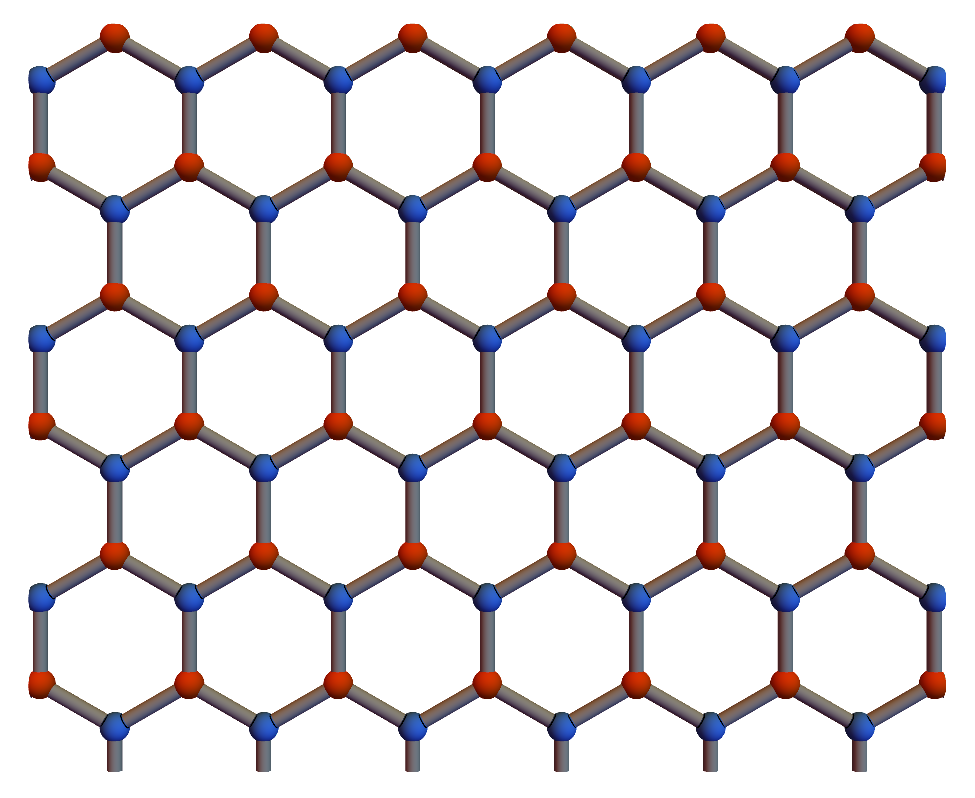
\includegraphics[width=\textwidth]{figs/CSL/MLG.pdf}
    \end{column}
\end{columns}
\end{frame}
%----------------------------------------------------------------------------------------
\begin{frame}{$J_1$ - $J_2$ $XY$ model on honeycomb lattice}
\begin{columns}
    \begin{column}{0.7\textwidth}
    \begin{block}{}
        \begin{equation*}
            \begin{pmatrix}
            J_2 (|f(\mathbf{k})|^2 - 3) & -J_1 f(\mathbf{k})\\
            -J_1 f^*(\mathbf{k}) & J_2 (|f(\mathbf{k})|^2 - 3)
            \end{pmatrix}
        \end{equation*}
        $$f(\mathbf{k}) = \sum_{\bm{\delta}} e^{i \mathbf{k} \bm{\delta}} = e^{-ik_x} + 2 e^{ik_x/2} \cos(\frac{\sqrt{3}}{2}k_y)$$
    \end{block}
    \begin{block}{}
        Eigenenergy: $E_{\pm} = \pm J_1 |f(\mathbf{k})| + J_2 |f(\mathbf{k})|^2 - 3t_2$

        \vspace{1cm}
        
        When $J_2 > J_1/6$, the minuma becomes a circle with radius $k_0 = \sqrt{2(1 - (J_1/6J_2)^2)}$
    \end{block}
    \end{column}
    
    \begin{column}{0.3\textwidth}  % Adjusted the column width
        \centering
        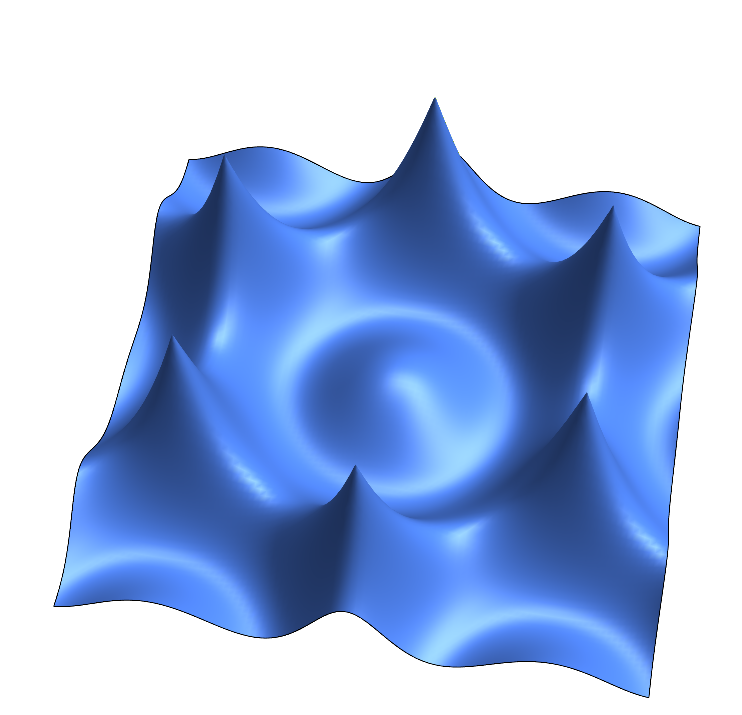
\includegraphics[width=\textwidth]{figs/CSL/graphene_moat.pdf}
    \end{column}
\end{columns}
\end{frame}
%----------------------------------------------------------------------------------------
\subsection{Fermionization}
%----------------------------------------------------------------------------------------
\begin{frame}{Fermionization}
    \begin{block}{}
        \begin{equation*} 
            S_{\mathbf{i}}^{+}
            =
            \exp(\sum_{j \ne i} i \theta_{ij} n_j) c_{\mathbf{i}}^{\dagger}
        \end{equation*}
        where $\theta_{ij} = \arg (\mathbf{r}_i - \mathbf{r}_j)$% is the relative angle between two sites
        ,
        %and 
        $c_{\mathbf{i}}^{\dagger}$ is the fermionic creation operators, $n_i = c_i^{\dagger} c_i$% is the particle number operators
    \end{block}

    \begin{block}{}
        \begin{equation*}
            H = -J_1 \sum_{<ij>} \exp(i\sum_{k}\phi_{ijk} n_k) c^{\dagger}_{i} c_{j} + J_2 \sum_{<<ij>>} \exp(i\sum_{k}\phi_{ijk} n_k) c^{\dagger}_{i} c_{j} + h.c.
        \end{equation*}
        where $\phi_{ijk} = \theta_{ik} - \theta_{jk}$% is the angle spanned by link $(i,j)$ with respect to point $k$
    \end{block}

    \begin{block}{}%Mean field solution
        At filling $\nu = \frac{1}{2n+1}$ with uniform density, ground state energy is minimized and ground state exhibits long-range entanglement in spin representation due to the gauge field (chiral spin liquid)
    \end{block}
\end{frame}
%----------------------------------------------------------------------------------------
\subsection{Low energy moat band model}
%----------------------------------------------------------------------------------------
\begin{frame}{Moat band and emergent CS gauge field}

\begin{columns}
    \begin{column}{0.7\textwidth}
        \begin{equation*}
            H = \int d\mathbf{r} \left[ \frac{1}{2M} \Phi^{\dagger}(\mathbf{r}) (|\mathbf{k}| - k_0)^2 \Phi(\mathbf{r}) + \frac{g}{M} [\Phi(\mathbf{r})^{\dagger} \Phi({\mathbf{r}})]^2 \right]
        \end{equation*}
        
        \begin{equation*}
            \eqnmarkbox[NavyBlue]{boson}{\Phi^{\dagger}(\bf r)} = \eqnmarkbox[OliveGreen]{fermion}{\Psi^{\dagger} (\bf r)} \eqnmarkbox[WildStrawberry]{flux}{\exp{i \int d{\bf r}' \arg({\bf r}' - {\bf r}) n({\bf r}')}}
        \end{equation*}
        \annotate[yshift=-0.5em]{below,left}{boson}{boson}
        \annotate[yshift=0.5em]{above, right}{fermion}{fermion}
        \annotate[yshift=-0.5em]{below, right}{flux}{CS phase}

        \vspace{2mm}
        \begin{block}{}
            \begin{equation*}
                H = \int d\mathbf{r} \left[ \frac{1}{2M} \Phi^{\dagger}(\mathbf{r}) (|\mathbf{k} - \mathbf{A}| - k_0)^2 \Phi(\mathbf{r}) \right]
            \end{equation*}
        % \end{block}
        
        % \begin{block}{}
            \begin{equation*}
                \mathbf{A}_\alpha(\mathbf{r})=\varepsilon_{\alpha\beta}\int d\mathbf{r}' \frac{(\mathbf{r}'-\mathbf{r})_\beta}{|\mathbf{r}'-\mathbf{r}|^2} n({\bf r}')
            \end{equation*}
            
            \begin{equation*}
                B(\mathbf{r})=\nabla \cross \mathbf{A}(\mathbf{r})=2\pi\int d\mathbf{r}' \delta(\mathbf{r}'-\mathbf{r}) n(\mathbf{r}') = 2\pi n(\mathbf{r})
            \end{equation*}
        \end{block}
    \end{column}
    
    % \begin{column}{0.3\textwidth}  % Adjusted the column width
    %     \centering
    %     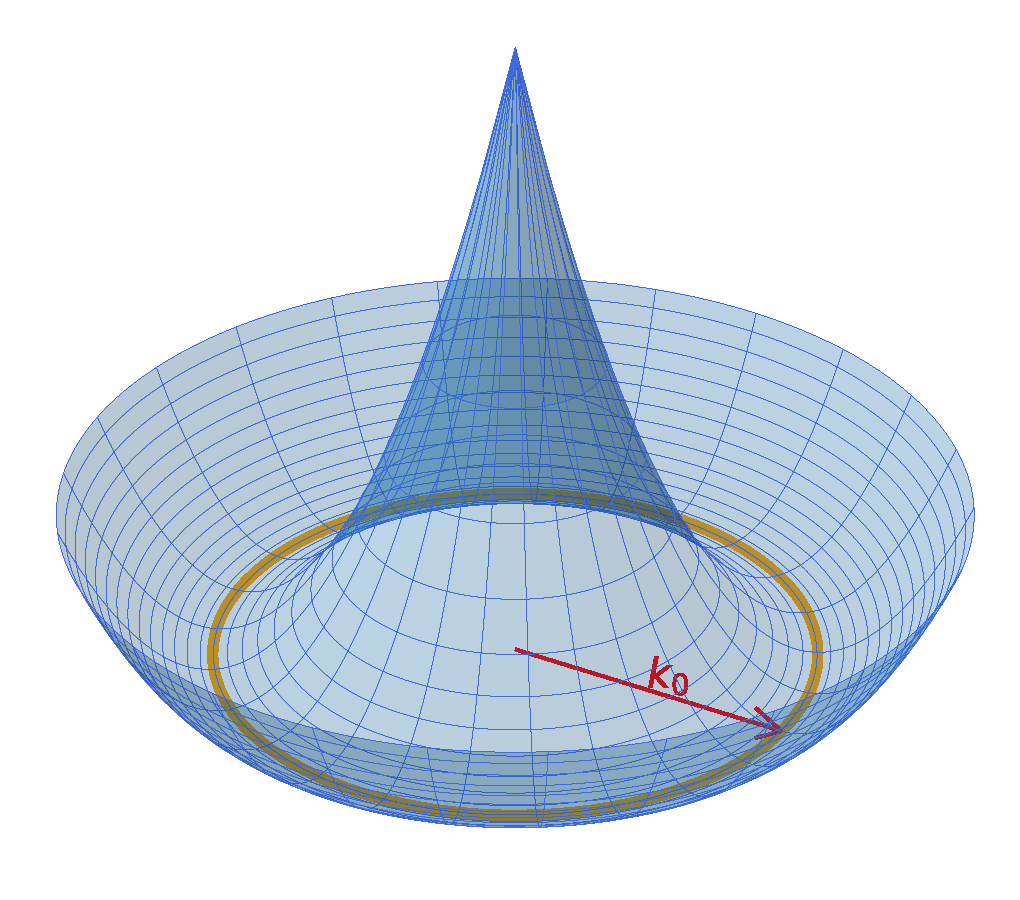
\includegraphics[width=\textwidth]{figs/CSL/moatband.pdf}
    % \end{column}
\end{columns}
\end{frame}
%----------------------------------------------------------------------------------------
\subsection{Variational energy}
%----------------------------------------------------------------------------------------
\begin{frame}{Variational energy}

\begin{columns}
    \begin{column}{0.6\textwidth}
    \begin{block}{}
        At low and uniform density $n \to 0$
        \begin{equation*}
            E \sim \langle k^2 \rangle - \langle |k| \rangle \sim \left(\frac{n}{n_0}\right)^2 \ln^2\left(\frac{n}{n_0}\right),
            \quad
            n_0 = \frac{k_0^2}{2\pi}
        \end{equation*}

        For comparison, energy per particle of BEC is
        % \begin{equation*}
            $E \sim gn {\rm ~or~} n^{4/3}$
        % \end{equation*}
    \end{block}
    \begin{block}{}
        Back to first quantization
        \begin{equation*}
            \Phi_B^{(l)} (z_1, z_2, \dots, z_N) = \prod_{i<j}^N \frac{z_i - z_j}{|z_i - z_j|} \Psi_F^{(l)} (z_1, z_2, \dots, z_N)
        \end{equation*}
        $\Psi_F^{(l)}$ is a Slater determinant
    \end{block}
    \end{column}
    \begin{column}{0.4\textwidth}
        \begin{figure}
            \centering
            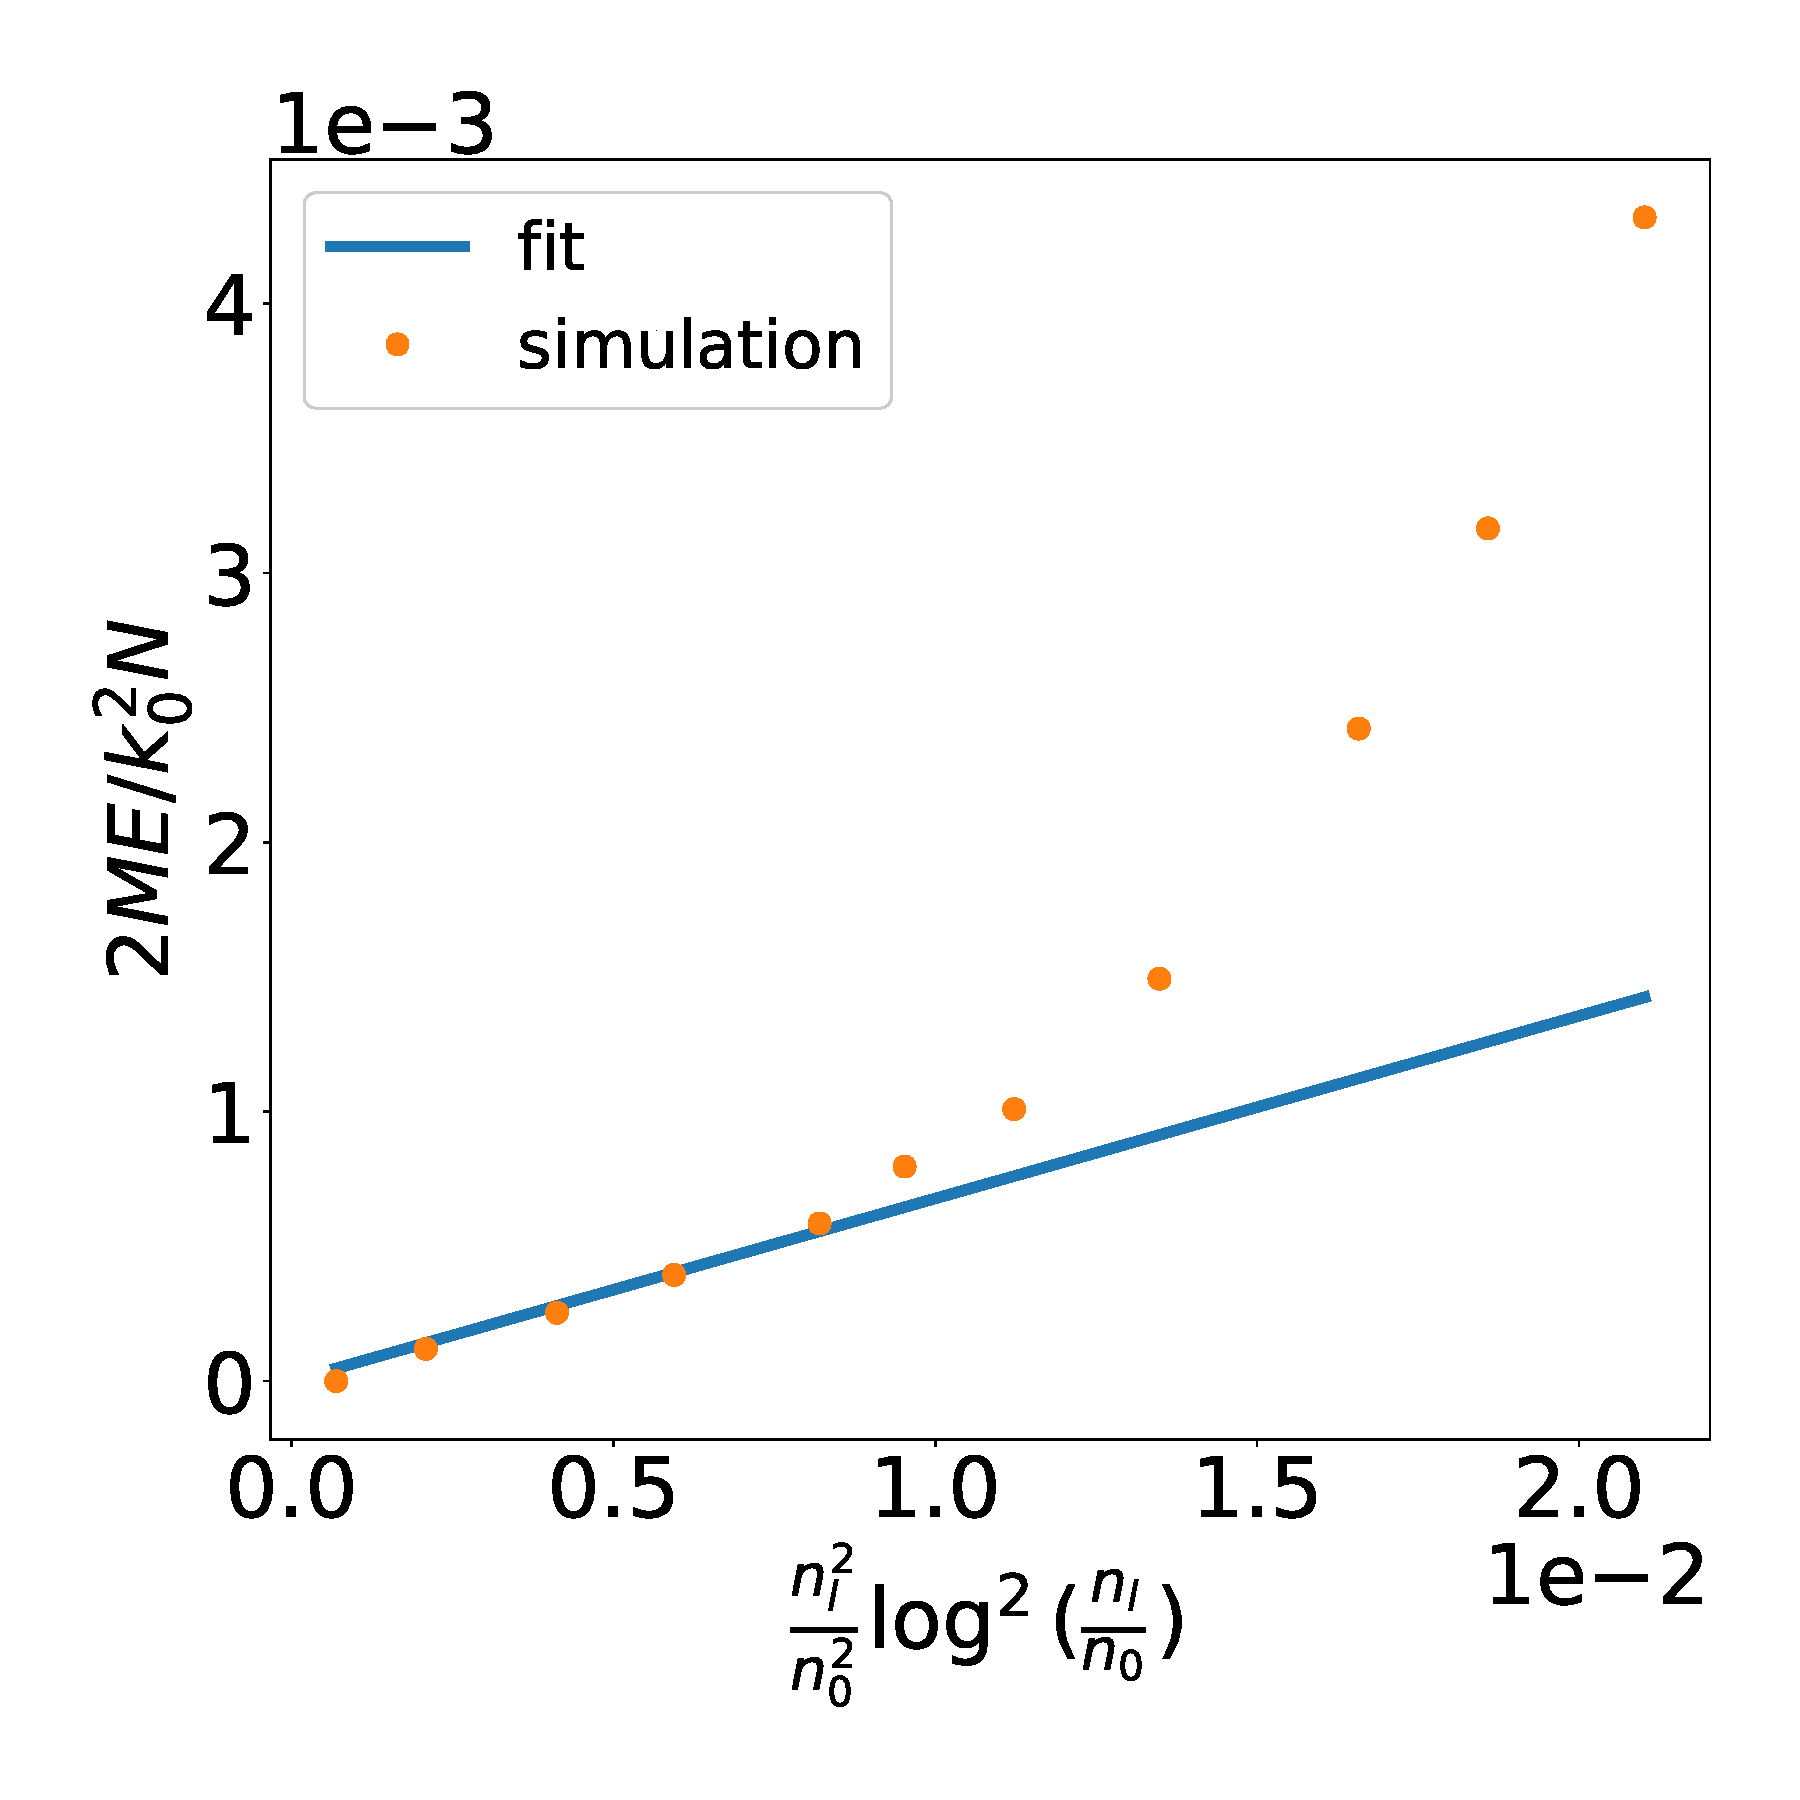
\includegraphics[width=\textwidth]{figs/CSL/Elown.pdf}
            \begin{picture}(0,0)
            {\def\unitlength{}
            \put(-0.35\textwidth,0.45\textwidth){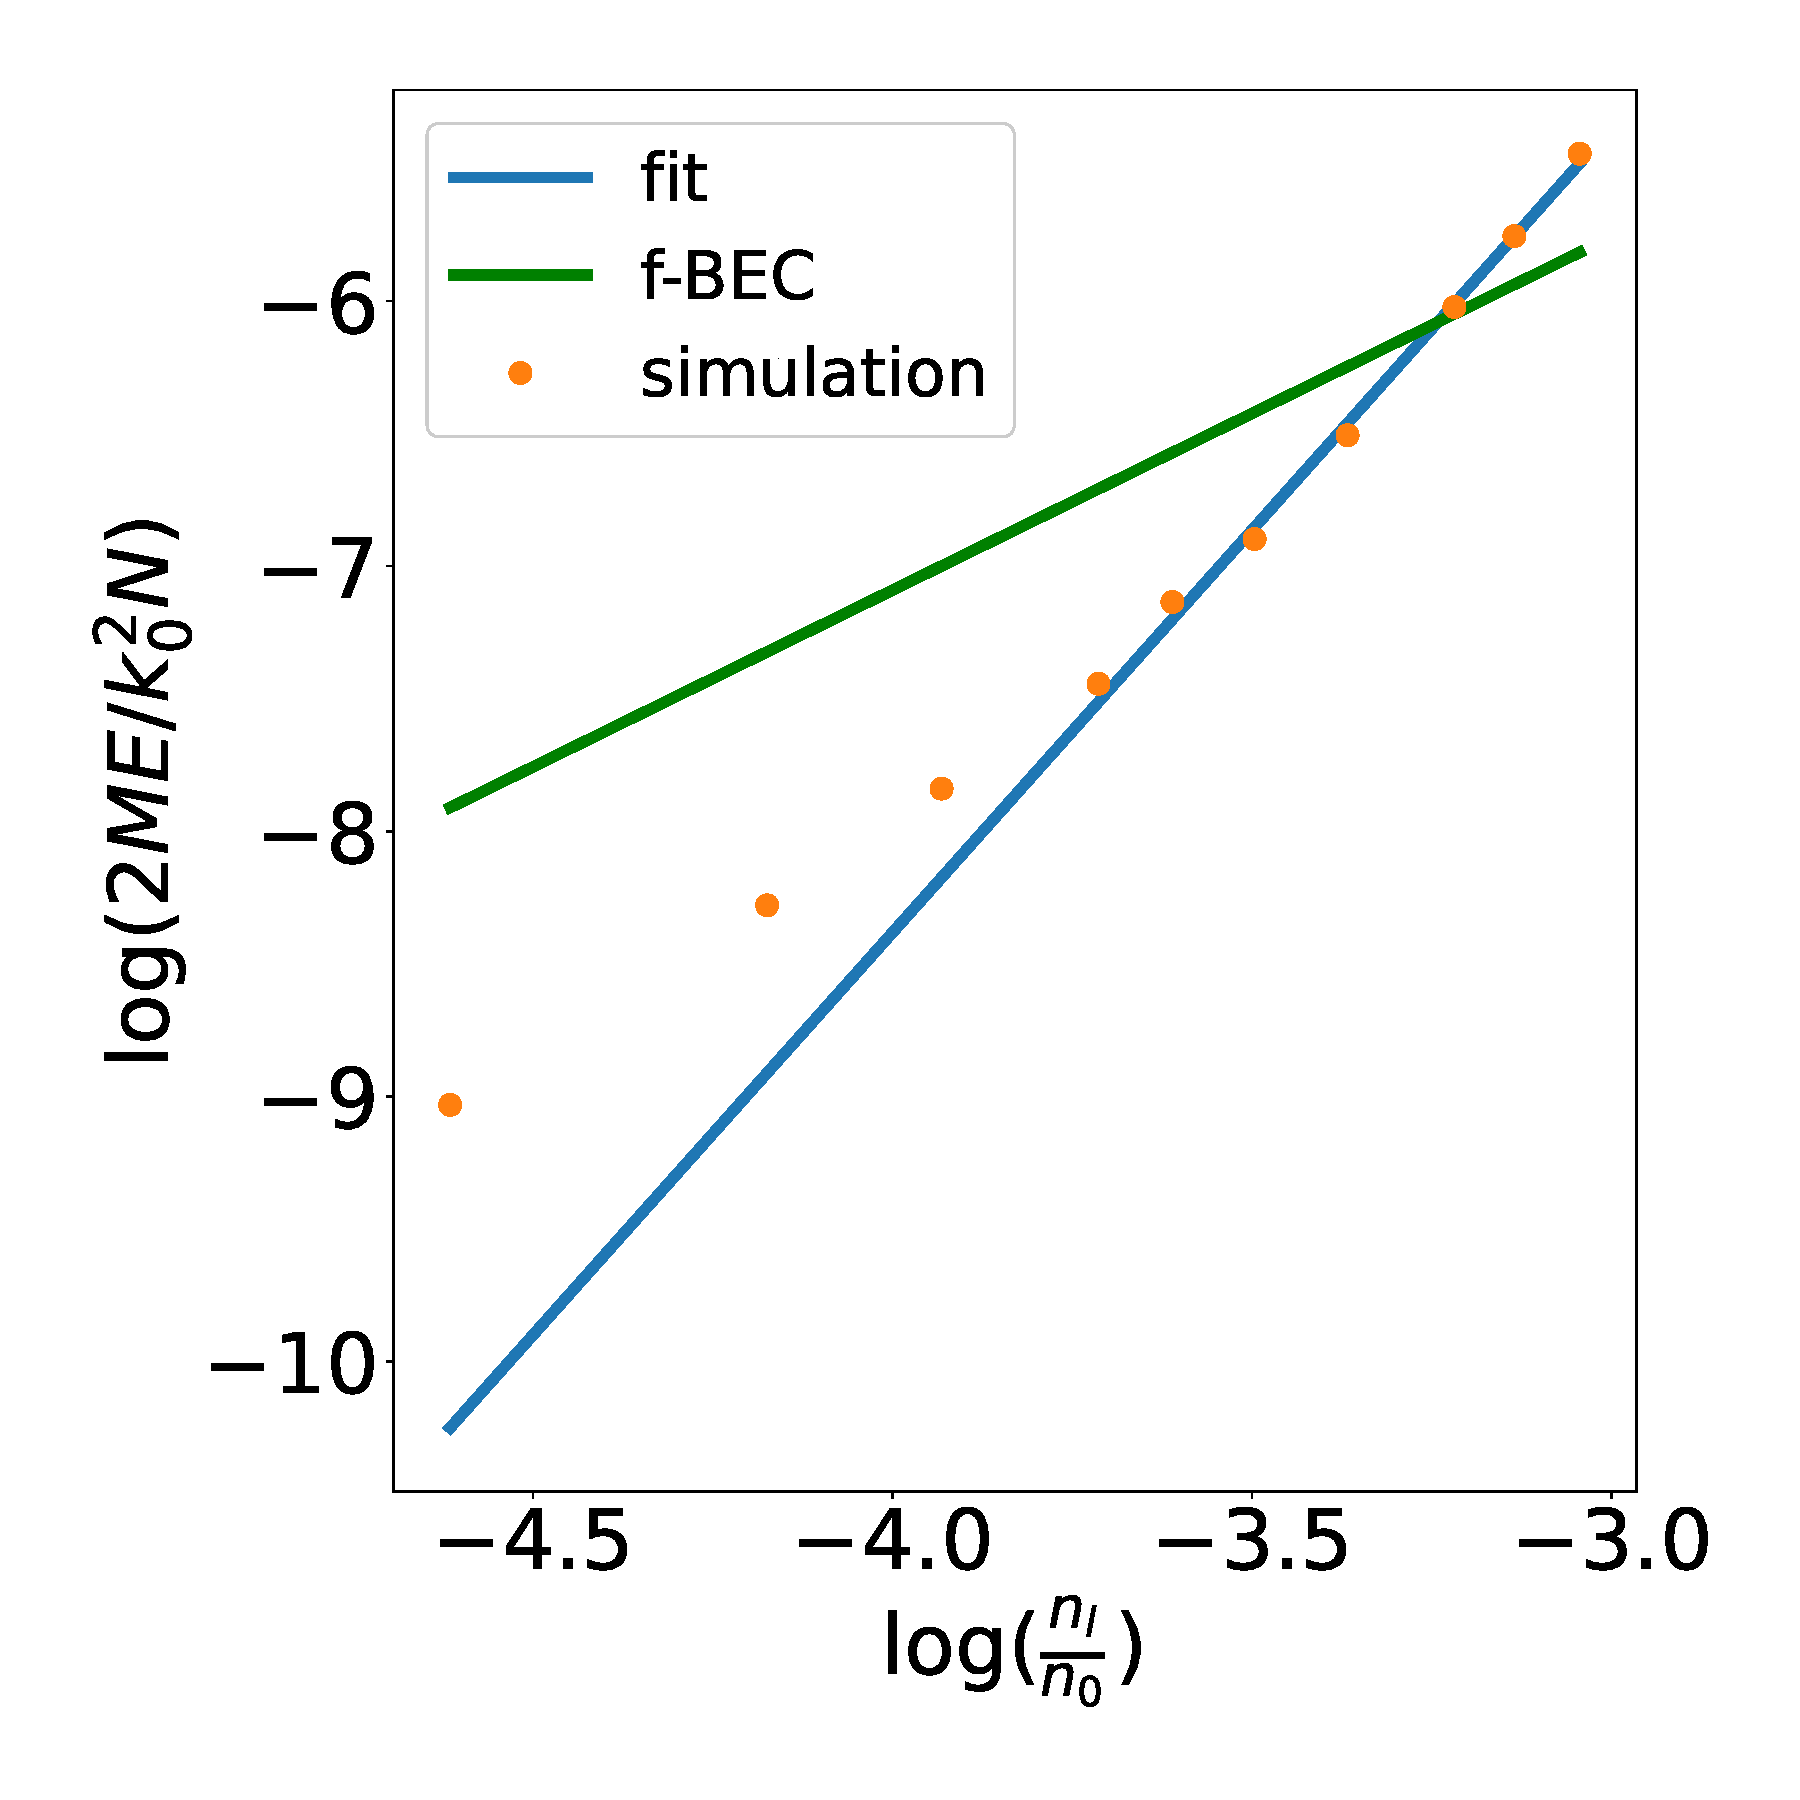
\includegraphics[height=0.4\textwidth]{figs/CSL/EhighnPow.pdf}}
            }
            \end{picture}
        \end{figure}
    \end{column}
\end{columns}

\end{frame}

%----------------------------------------------------------------------------------------
\subsection{Phase diagram}
%----------------------------------------------------------------------------------------
\begin{frame}{Phase diagram}
\begin{columns}
\begin{column}{0.4\textwidth}
\begin{figure}
    \centering
    \begin{minipage}{1.0\linewidth}
    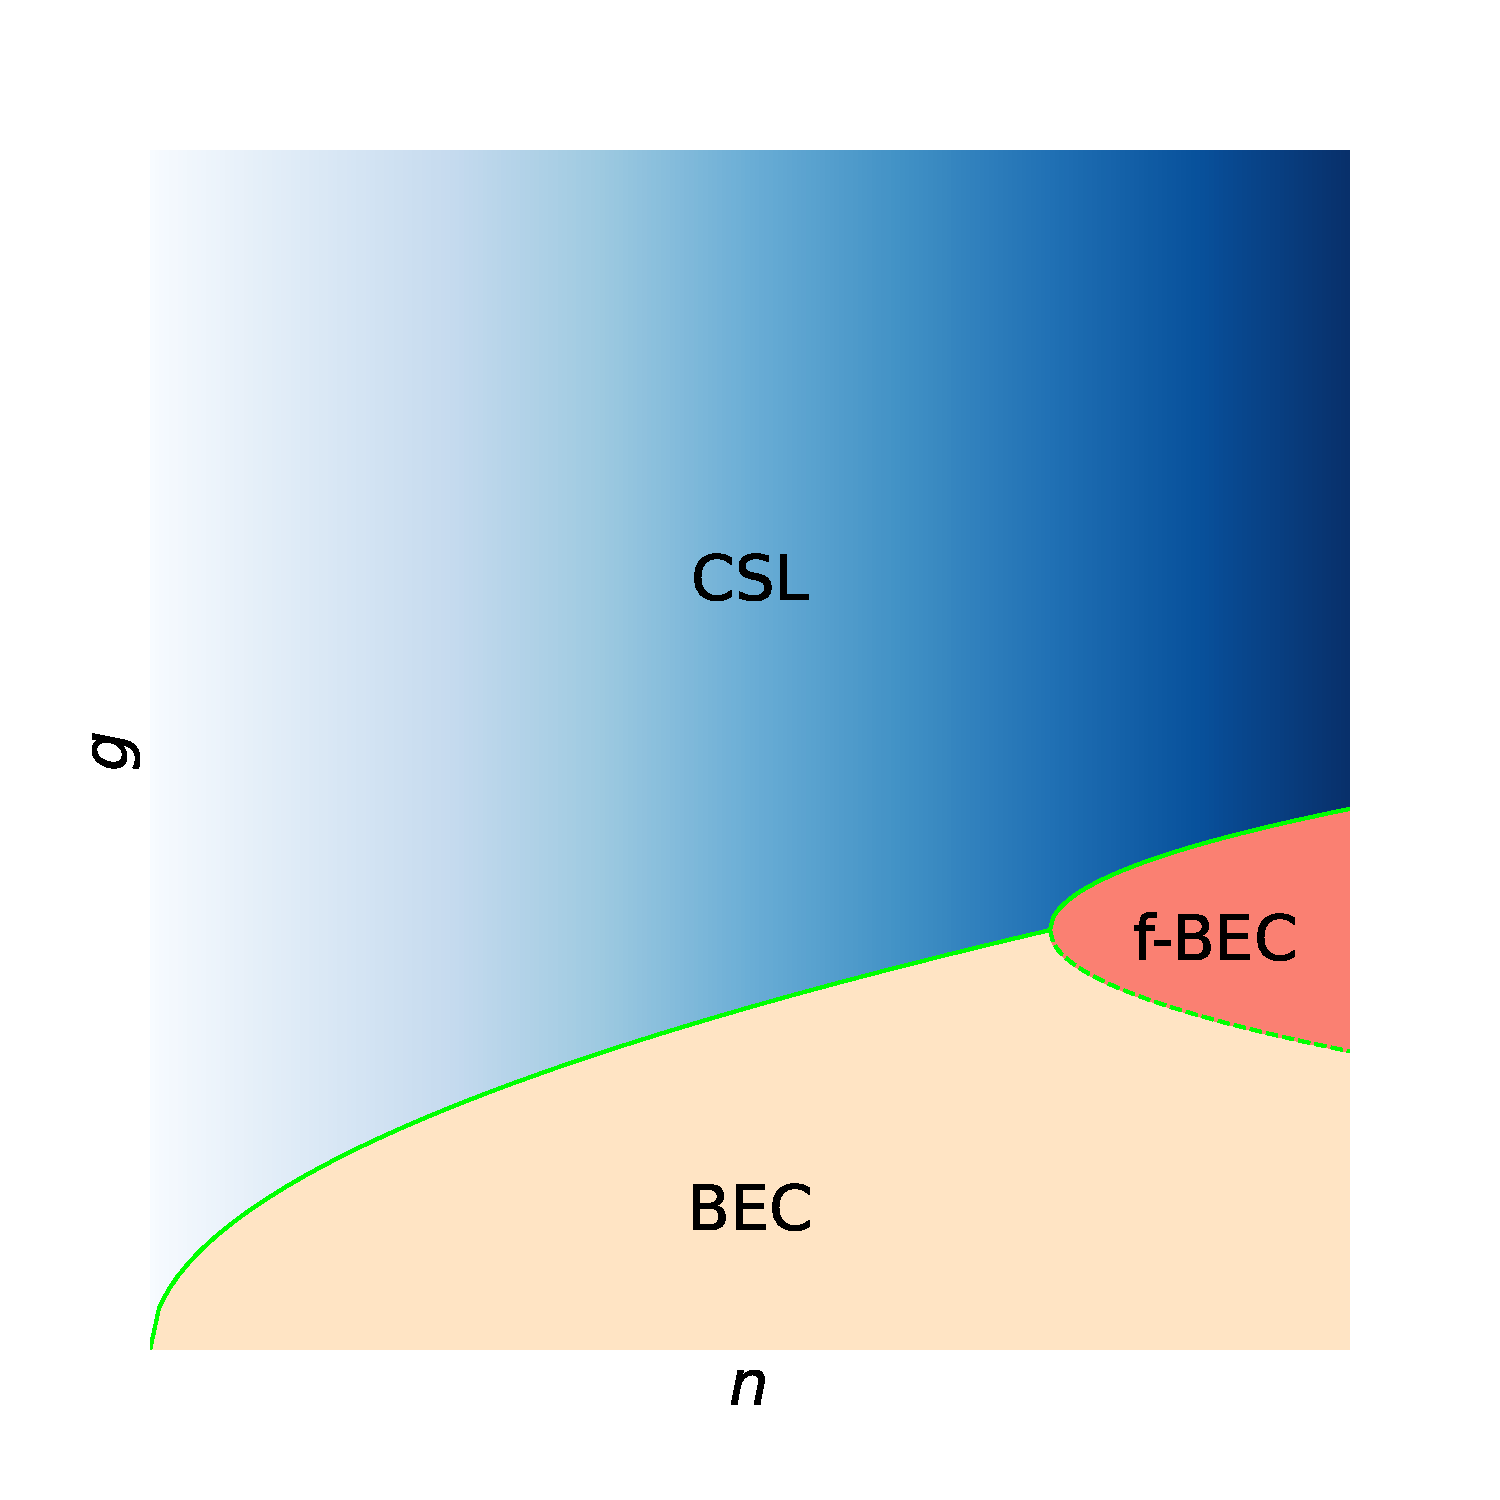
\includegraphics[width=\linewidth]{figs/CSL/PD.pdf}
    \begin{picture}(0,0)
    {\def\unitlength{}
    \put(0.44\textwidth,0.38\textwidth){\tiny $U(1)$ symmetry}
    \put(0.49\textwidth,0.35\textwidth){\tiny breaking}
    \put(0.61\textwidth,0.4\textwidth){\vector(2,1){0.12\textwidth}}
    \put(0.58\textwidth,0.35\textwidth){\vector(-2,-1){0.1\textwidth}}
    % \put(0.42\textwidth,0.68\textwidth){$E \sim n^{3.0}$}
    % \put(0.68\textwidth,0.82\textwidth){$E \sim n^{4/3}$}
    % \put(0.63\textwidth,0.3\textwidth){$E \sim gn$}
    \multiput(0.427\textwidth,0.19\textwidth)(0\textwidth,0.04\textwidth){20}{\line(0,1){0.02\textwidth}}
    \multiput(0.7\textwidth,0.19\textwidth)(0\textwidth,0.04\textwidth){7}{\line(0,1){0.02\textwidth}}
    \put(0.41\textwidth,0.1\textwidth){$n^*_1$}
    \put(0.62\textwidth,0.1\textwidth){$n^*_2 \sim 1.64n^*_1$}
    \put(0.25\textwidth,0.79\textwidth){\tiny Non-uniformity increasing}

    \multiput(0.11\textwidth,0.465\textwidth)(0.04\textwidth,0\textwidth){15}{\line(1,0){0.02\textwidth}}
    \put(0\textwidth,0.39\textwidth){$g \sim 1$}

    \begin{tikzpicture}[overlay]
        \node[draw, single arrow,
              minimum height=0.6\textwidth, minimum width=0.1\textwidth,
              single arrow head extend=0.02\textwidth,
              anchor=west, rotate=0] at (0.2\textwidth,0.8\textwidth) {};
    \end{tikzpicture}
    }
    \end{picture}
    % \phantomsubcaption{\label{fig:}}
    \end{minipage}
\end{figure}
\end{column}

\begin{column}{0.6\textwidth}
    \begin{itemize}
        \item Non uniformity could appear at large density. For interaction strength $g = 1$, MC simulation indicates the boundary $n^*_1=k^2_0 / 82 \pi$.

        \vspace{5mm}
        
        \item f-BEC could appear at interaction strength $g$ of order $1$, and $n^*_2=k^2_0 / 50 \pi$ sets the boundary.
    \end{itemize} 
\end{column}
\end{columns}
\end{frame}